% !TEX encoding = UTF-8 Unicode
\documentclass[12pt,a4paper,english
% ,twoside,openright
]{tunithesis}

\special{papersize=210mm,297mm}

\author{Roosa Kuusivaara \& Väinö-Waltteri Granat}
\title{Digital Image Formation And Processing - Report} % primary title (for front page)
\thesistype{Laboratory Report} % or Bachelor of Science, Laboratory Report...

\usepackage{graphicx}

\usepackage{lastpage}
\usepackage[english]{babel}
\usepackage[
backend=biber,
style=numeric,
citestyle=numeric,
autocite=inline
]{biblatex}
\usepackage{csquotes}
\usepackage{matlab-prettifier}
\usepackage{svg}

\addbibresource{references.bib} %Imports bibliography file


\definecolor{tunipurple}{RGB}{78, 0, 142}

\newcommand\todo[1]{{\color{red}!!!TODO: #1}} % Remark text in braces appears in red
\newcommand{\angs}{\textsl{\AA}}              % , e.g. slanted symbol for Ångstöm
% Preparatory content ends here


\pagenumbering{roman} % was: {Roman}
\pagestyle{headings}
\begin{document}

% Special trick so that internal macros (denoted with @ in their name)
% can be used outside the cls file (e.g. \@author)
\makeatletter

% Create the title page.
% First the logo. Check its language.
\thispagestyle{empty}
\vspace*{-.5cm}\noindent

\begin{figure}
    \vspace{-1.3cm}
    \advance\leftskip-2.5cm
    \noindent
\includegraphics{img/tunilogo.png}
\end{figure}
 
\vspace{2.5cm}
\begin{flushright}
\noindent\textsf{\LARGE{\@author}}

\noindent\vspace{0.5cm}

\noindent\Huge{\textsf{\textbf{\textcolor{tunipurple}{\@title}}}}
\end{flushright}
\vspace{13.7cm} % adjust to 12.7 this if thesis title needs two lines

% Last some additional info to the bottom-right corner
\begin{flushright}  
    \begin{spacing}{1.0}
      \textsf{Faculty of Information Technology and Communication Sciences (ITC)\\
      \@thesistype\\}
    \end{spacing}
\end{flushright}

% Leave the backside of title page empty in twoside mode
\if@twoside
\clearpage
\fi

% Turn off page numbering for the first pages
\pagenumbering{gobble}


% Some fields in abstract are automated, namely those with \@ (author,
% title, thesis type).
\chapter*{Abstract}
\begin{spacing}{1.0}
\noindent \@author: \@title\\
\@thesistype\\
Tampere University\\
Master’s Degree Programme in Signal Processing\\
December 2023
\end{spacing}
\noindent\rule{12cm}{0.4pt}

\vspace{0.5cm}

% ---------------------------------------
% Abstract and keywords
% ---------------------------------------

\noindent
This report documents the work done in the Digital Image Formation And Processing assignment as a part of the Advanced signal processing laboratory course. In this assignment we familiarized ourselves with basics of digital image formation from raw sensor data as well as image processing.

~

\noindent\textbf{Keywords:} Image processing, Image formation.

~

\noindent The originality of this thesis has been checked using the Turnitin Originality Check service.


% Add the table of contents


\setcounter{tocdepth}{3}              % How many header level are included
\tableofcontents                      % Create TOC


% The actual text begins here and page numbering changes to 1,2...
% Leave the backside of title empty in twoside mode
\if@twoside
%\newpage
\cleardoublepage
\fi


\renewcommand{\chaptername}{} % This disables the prefix 'Chapter' or
                              % 'Luku' in page headers (in 'twoside'
                              % mode)


\chapter{Introduction}
\label{ch:intro} 
In this report we describe our work done in the 'Digital Image Formation and Processing' laboratory assignment for the Advanced Signal Processing Laboratory course. In this assignment we implemented a basic raw image formation and processing pipeline in Matlab to construcut RGB images from raw sensor data.

\pagenumbering{arabic}
\setcounter{page}{1} 

\chapter{Methodology}
\label{sec:methodology}
In this section we will present our implementation of the image processing pipeline, by going over the main parts of the Matlab code as well as explaining the the decisions we took when requirements we ambigious.

\section{Overview of the pipeline}
Figure~\ref{fig:pipeline} shows the complete image processing and formation pipeline that we are going to introduce in this report. The following sections will go over the different parts of the pipeline. The pipeline takes in raw sensor data of Bayer arrays in RGGB format and produces RGB images. In addition to image formation the pipeline also performs focusing, white balancing and contrast and saturation correction.

\begin{figure}
  \centering
  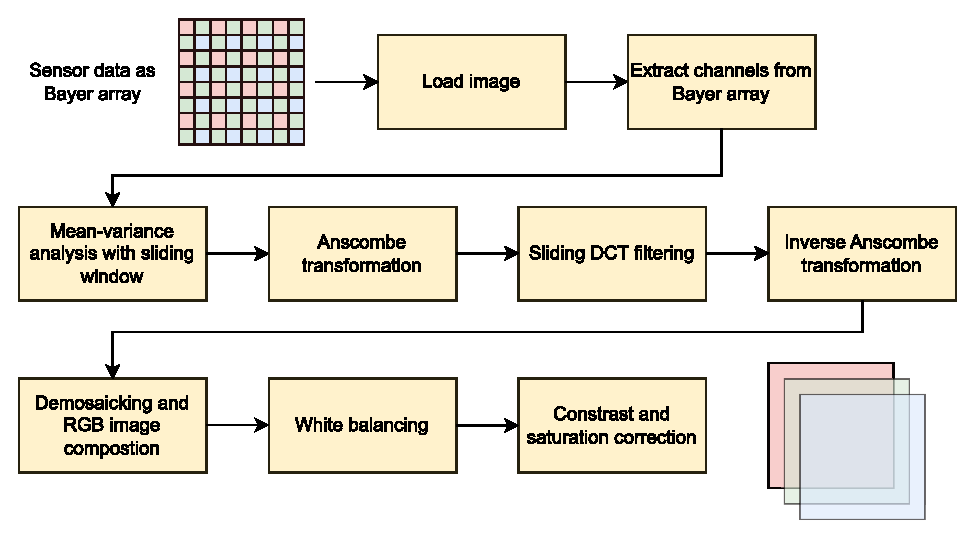
\includegraphics[width=0.8\textwidth]{img/image_pipeline.eps}
  \caption{Our image processing and formation pipeline}
  \label{fig:pipeline}
\end{figure}

\section{Reading images and converting to doubles}
The first part of the pipeline is loading the images (outoffocus.tiff and natural.tiff) using Matlab's $imread$ function, and then converting the pixel values to double precision by using $im2double$ function. The convertion ensure that pixel values are represented as floating-point numbers between 0 and 1. 
\begin{lstlisting}[style=Matlab-editor, numbers=left, basicstyle=\small]
% 1. Load image and convert to double
focus = imread('images/outoffocus.tiff');
focus = im2double(focus);

natural = imread('images/natural.tiff');
natural = im2double(natural);
\end{lstlisting}

\section{Image visualization and Bayer mosaic}
The second part starts with creating a figure with two subplots. The $imshow$ function is used with $[]$ to scale the pixel values automatically for better visualization. For illustrating the Bayer mosaic arrays the image is separated into its color channels (red, green 1, green 2 and blue). After separating the color channels, the next step is to create figures to illustrate the Bayer mosaic arrays for each color channel separately.
\begin{lstlisting}[style=Matlab-editor, numbers=left, basicstyle=\small]
% 2. Visualize Images, Bayer mosaic array
% Define the block size
figure;
subplot(1,2,1); imshow(focus, []); title('out of focus image');
subplot(1,2,2); imshow(natural, []); title('natural');

% 3. Separe image into subchannels
R_focus = focus(1:2:end, 1:2:end);
G1_focus = focus(1:2:end, 2:2:end);
G2_focus = focus(2:2:end, 1:2:end);
B_focus = focus(2:2:end, 2:2:end);

R_nat = natural(1:2:end, 1:2:end);
G1_nat = natural(1:2:end, 2:2:end);
G2_nat = natural(2:2:end, 1:2:end);
B_nat = natural(2:2:end, 2:2:end);

% Illustrare the bayer array

% Plot channels
figure;
subplot(2,2,1); imshow(R_focus, []); title('Red');
subplot(2,2,2); imshow(G1_focus, []); title('Green 1');
subplot(2,2,3); imshow(G2_focus, []); title('Green 2');
subplot(2,2,4); imshow(B_focus, []); title('Blue');
sgtitle("Out of focus image");

figure;
subplot(2,2,1); imshow(R_nat, []); title('Red');
subplot(2,2,2); imshow(G1_nat, []); title('Green 1');
subplot(2,2,3); imshow(G2_nat, []); title('Green 2');
subplot(2,2,4); imshow(B_nat, []); title('Blue');
sgtitle("Natural image");
\end{lstlisting}
\section{Sliding window}
In this section we are analyzing each subchannel of the out-of-focus and natural images using a sliding window operator. For both natural image and out-of-focus image we are calling \texttt{calculateScatterPlot} function for each color channel.

The function defines a sliding window analysis using the \texttt{blockproc} function in Matlab. The window size is set to $[2, 2]$, and $calculateMeanVar$ function is defined to calculate the mean and variance for each window. The function $calculateScatterPlot$ returns mean values and variance values that we need in the next step when calculating regression lines.

\begin{lstlisting}[style=Matlab-editor, numbers=left, basicstyle=\small]
% 4. Calculate scatter plots
function [meanValues, varianceValues] = calculateScatterPlot(channel)
    % Define the window size for sliding window analysis
    windowSize = [2, 2];

    % Define a function to calculate mean and variance for each window
    calculateMeanVar = @(block_struct) [mean(block_struct.data(:)), var(block_struct.data(:))];

    % Apply the sliding window operator using blockproc
    meanVarResults = blockproc(channel, windowSize, calculateMeanVar);

    % Extract mean and variance values
    meanValues = meanVarResults(:, 1);
    varianceValues = meanVarResults(:, 2);

    % Reshape the results for scatterplot creation
    meanValues = meanValues(:);
    varianceValues = varianceValues(:);
end
\end{lstlisting}

\section{Scatterplots and regression}
In this part we calculate the regression lines for each subchannel using the \texttt{calculateRegression} function. Regression is calculated by $polyfit$ function in Matlab, that returns a best-fitting polynomial to a set of data points, in this context it is used to fit a straight line to the data. The regression calculation will be done for both out-of-focus and natural subchannels.
\begin{lstlisting}[style=Matlab-editor, numbers=left, basicstyle=\small]
% 5. Calculate regression lines
function [p] = calculateRegression(meanValues, varianceValues)
    % Fit a straight line to the data
    p = polyfit(meanValues, varianceValues, 1);
end
\end{lstlisting}
Then,  \texttt{produceScatterPlot} function is responsible for generating scatter plots for each color channel of the out-of-focus image. This function takes as input the mean values and variance values obtained from the \texttt{calculateScatterPlot} function, as well as the regression lines calculated by the \texttt{calculateRegression} function. After running this function, you should have scatter plots with regression lines for each subchannel.

\begin{lstlisting}[style=Matlab-editor, numbers=left, basicstyle=\small]
function produceScatterPlot(meanR, varR, pR, meanG1, varG1, pG1, meanG2, varG2, pG2, meanB, varB, pB)
    % Create a new figure
    figure;
    
    % Fit a straight line to the Red channel data and plot it
    subplot(2,2,1);
    scatter(meanR, varR);
    xlabel('Local Sample Mean');
    ylabel('Local Sample Variance');
    title('Mean-Variance Scatterplot for Red');
    hold on;
    fR = polyval(pR, meanR);
    plot(meanR, fR, 'r');
    hold off;
    
    % Fit a straight line to the Green 1 channel data and plot it
    subplot(2,2,2);
    scatter(meanG1, varG1);
    xlabel('Local Sample Mean');
    ylabel('Local Sample Variance');
    title('Mean-Variance Scatterplot for Green 1');
    hold on;
    fG1 = polyval(pG1, meanG1);
    plot(meanG1, fG1, 'g');
    hold off;

    % Fit a straight line to the Green 2 channel data and plot it
    subplot(2,2,3);
    scatter(meanG2, varG2);
    xlabel('Local Sample Mean');
    ylabel('Local Sample Variance');
    title('Mean-Variance Scatterplot for Green 2');
    hold on;
    fG2 = polyval(pG2, meanG2);
    plot(meanG2, fG2, 'g');
    hold off;
    
    % Fit a straight line to the Blue channel data and plot it
    subplot(2,2,4);
    scatter(meanB, varB);
    xlabel('Local Sample Mean');
    ylabel('Local Sample Variance');
    title('Mean-Variance Scatterplot for Blue');
    hold on;
    fB = polyval(pB, meanB);
    plot(meanB, fB, 'b');
    hold off;
end
\end{lstlisting}

\section{Transformation and inverse transformation}
[kesken]

Transformation is done by using this equation
\[
2 \sqrt{\frac{I_c}{a_c} + \frac{3}{8} + \frac{b_c}{a_c^2}}
\],
 where $a_c$ and $b_c$ are the parameters estimated from the out-of-focus image.

\begin{lstlisting}[style=Matlab-editor, numbers=left, basicstyle=\small]
% 6. Transformation
function output = applyTransformation(block_struct, ac, bc)
    % Calculate the value inside the square root
    sqrt_val = (block_struct.data / ac) + (3/8) + (bc / (ac^2));

    % Check if the value inside the square root is negative
    sqrt_val(sqrt_val < 0) = 1;

    % Calculate the output
    output = 2 * sqrt(sqrt_val);
end
\end{lstlisting}

The inverse transformation is done by using the equation
\[
a_c \left( \frac{1}{4} D^2 + \frac{1}{4}\sqrt{\frac{3}{2}D^{-1}} - \frac{11}{8}D^{-2} + \frac{5}{8}\sqrt{\frac{3}{2}D^{-3}} - \frac{1}{8} - \frac{b_c}{a_c^2} \right)
\]
\begin{lstlisting}[style=Matlab-editor, numbers=left, basicstyle=\small]
% % 9. Inverse transformation
function output = inverseTransformation(block_struct, ac, bc)
    % Calculate the values inside the square roots
    sqrt_val1 = 0.25 * sqrt(3/2) * block_struct.data.^(-1);
    sqrt_val2 = (5/8) * sqrt(3/2) * block_struct.data.^(-3);

    % Check if the values inside the square roots are negative
    sqrt_val1(block_struct.data.^(-1) < 0) = 0;
    sqrt_val2(block_struct.data.^(-3) < 0) = 0;

    % Calculate the output
    output = ac * (0.25 * block_struct.data.^2 + ...
        sqrt_val1 - ...
        (11/8)*(block_struct.data.^(-2)) + ...
        sqrt_val2 - ...
        1/8 - ...
        bc/(ac^2));
end
\end{lstlisting}

\section{DCT denoising}
This part implements a denoising operation on an image using a sliding DCT (Discrete Cosine Transform) filter. The DCT image denoising applies to each subchannel of both the original and transformed versions of the natural image. The \texttt{DCTImageDenoising} function takes an image, a threshold parameter $\lambda$ and the block size for the DCT operation. For the threshold parameter $\lambda$ we selected 0.060 for getting the most visually convincing result. The block size used is [8 8]. The \texttt{thresholdDCT} function applies the DCT to a given block of the image, thresholds the DCT coefficients by setting values below a threshold $\lambda$ to zero, and then returns the denoised block.

\begin{lstlisting}[style=Matlab-editor, numbers=left, basicstyle=\small]
function [denoised] = DCTImageDenoising(image, lambda, transformBlockSize)

    % Create a custom function to be applied to each block
    fun = @(block_struct) idct2(thresholdDCT(block_struct.data, lambda));

    % Apply the function to each block
    denoised = blockproc(image, transformBlockSize, fun);
end

function denoised = thresholdDCT(input, lambda)

    % Apply DCT to the block
    dctBlock = dct2(input);

    % Threshold the DCT coefficients
    dctBlock(abs(dctBlock) < lambda) = 0;
    denoised = dctBlock;
end
\end{lstlisting}

\section{Demosaicking}
This section performs a simple demosaicking operation using linear interpolation. After running the function \texttt{simpleDemosaic}, it creates a full-color RGB image from the color channels by interpolating the missing color information between pixels in the Bayer mosaic pattern. For interpolation we use $interp2$ function in Matlab and nearest-neighbour method.

\begin{lstlisting}[style=Matlab-editor, numbers=left, basicstyle=\small]
function [output] = simpleDemosaic(R, G1, G2, B)

    % Define output array;
    R_out = zeros(size(R)*2);
    G1_out = zeros(size(R)*2);
    G2_out = zeros(size(R)*2);
    B_out = zeros(size(R)*2);

    % Get the size of the images
    [M, N] = size(R_out);

    % Create a meshgrid for interpolation
    [Xout, Yout] = meshgrid(1:N, 1:M);

    % Shift the grids for each channel according to the Bayer pattern
    [Xr, Yr] = meshgrid(1:2:N, 1:2:M);
    [Xg1, Yg1] = meshgrid(1:2:N, 2:2:M);
    [Xg2, Yg2] = meshgrid(2:2:N, 1:2:M);
    [Xb, Yb] = meshgrid(2:2:N, 2:2:M);

    % Interpolate the images
    r_interp = interp2(Xr, Yr, R, Xout, Yout, 'nearest', 0);
    g1_interp = interp2(Xg1, Yg1, G1, Xout, Yout, 'nearest', 0);
    g2_interp = interp2(Xg2, Yg2, G2, Xout, Yout, 'nearest', 0);
    b_interp = interp2(Xb, Yb, B, Xout, Yout, 'nearest', 0);

    g_interp = (g1_interp + g2_interp)/2;

    output = cat(3, r_interp, g_interp, b_interp);
end
\end{lstlisting}


\section{White balancing}
The purpose of white balancing is to correct the color cast in an image so that the white color appears neutral. The \texttt{whiteBalance} function implements basic white balancing method by identifying the pixel with maximum intensity in the image and and then normalizes the entire image by dividing each RGB pixel by the RGB values of the maximum intensity pixel. 
\begin{lstlisting}[style=Matlab-editor, numbers=left, basicstyle=\small]
function balancedImage = whiteBalance(image)

% Check the range of the image data
minVal = min(image(:));
maxVal = max(image(:));

% If the range is not [0, 1], scale the image data
if minVal < 0 || maxVal > 1
    image = (image - minVal) / (maxVal - minVal);
    max(image, [], 'all')
end

% Convert to HSV
hsvImg = rgb2hsv(image);

% Find location of maximum intensity from the hsv representation
maxPixelValue = max(hsvImg(:,:,3), [], 'all');
[x,y] = find(hsvImg(:,:,3)==maxPixelValue, 1, 'first');

% Divide all the pixel by the found pixel in rgb space
balancedImage(:,:,1) = image(:,:,1) ./ image(x,y,1);
balancedImage(:,:,2) = image(:,:,2) ./ image(x,y,2);
balancedImage(:,:,3) = image(:,:,3) ./ image(x,y,3);

% Prevent values over limits
balancedImage = min(max(balancedImage, 0), 1);

end
\end{lstlisting}

\section{Contrast and saturation correction}
The last part of our pipeline involves contrast and saturation correction. The correction is applied using the \texttt{contrastAndSaturationCorrection} function and takes the image and a gamma value as inputs. The gamma value influences the degree of saturation correction, allowing a visual enhancement. For the correlation, the image is converted to the HSV color space, because then the function can focus on contrast adjustment in the V channel and saturation correction in the S channel.

\begin{lstlisting}[style=Matlab-editor, numbers=left, basicstyle=\small]
function img_corrected = contrastAndSaturationCorrection(img, gamma_value)
    % Convert the image to the HSV color space
    img_hsv = rgb2hsv(img);

    % Perform histogram equalization on the V channel for contrast correction
    img_hsv(:,:,3) = histeq(img_hsv(:,:,3));

    % Perform gamma correction on the S channel for saturation correction
    img_hsv(:,:,2) = img_hsv(:,:,2).^gamma_value;

    % Convert the image back to the RGB color space
    img_corrected = hsv2rgb(img_hsv);
end
\end{lstlisting}


\chapter{Results}
\label{sec:results}
In this section we will present the results from our image processing pipeline and also do some analysis on why we got the kinds of results that we did.


\section{Purpose of the Anscombe transformation}
In image processing Poisson distribution is used to model the signal dependant noise specific in images, due to it better model photons hitting the sensor array then Gaussian distribution. Gaussian distribution is signal independant and thus more suitable for general purpose denoising methods, so we want to transform our image specific Poisson noise to corresponding Gaussian distribution for processing. This is accomplished with the Anscombe transformation. After denoising we can use the inverse Anscombe transformation to bring the image back to Poisson noise distribution where the image should now appear denoised.

Equation~\ref{eq:anscombe} shows the Anscombe transformation and equation~\ref{eq:anscombe-inv} shows the function used to inverse the Anscombe transformation. Where $a_{c}$ and $b_{c}$ describe the variance of noise in the image and $D$ denotes the denoised image. For the purposes of this exercise the inversing function is not exactly the same as inverse Anscombe tranformations. According to~\cite{poissonnoise2011} and~\cite{poissonnoise2011-2} this is because for images with low intensity (lesser frequency) the precise inverse function performs poorly due to bias caused by the non-linear forward function.

\begin{equation}
\label{eq:anscombe}
  2 \sqrt{\frac{I_{c}}{a_{c}} + \frac{3}{8} + \frac{b_{c}}{a_{c}^2}}
\end{equation}

\begin{equation}
\label{eq:anscombe-inv}
  a_{c} \Bigg( \frac{1}{4}D^2 + \frac{1}{4}\sqrt{\frac{3}{2}}D^{-1} - \frac{11}{8}D^{-2} + \frac{5}{8} \sqrt{\frac{3}{2}}D^{-3} - \frac{1}{8} - \frac{b_{c}}{a_{c}^2} \Bigg)
  \end{equation}

\section{Mean variance analysis}
With a sliding window mean and variance operators we could extract local noise information from the out of focus image to visualize how the Anscombe transformation affects the image. Figure~\ref{fig:noisy-mean-variance} shows the local means and variances for each channel as datapoints and the affine variance as colored lines before the Anscombe transformation. From the lines we see that they are not flat like we would expect. Figure~\ref{fig:clean-mean-variance} shows the same image after the Anscombe transformation. We can now see that the regressions lines are flat. This is because the Anscombe transformation has made the signal dependant noise (Poisson noise) a constant troughout the image.

\begin{figure}
  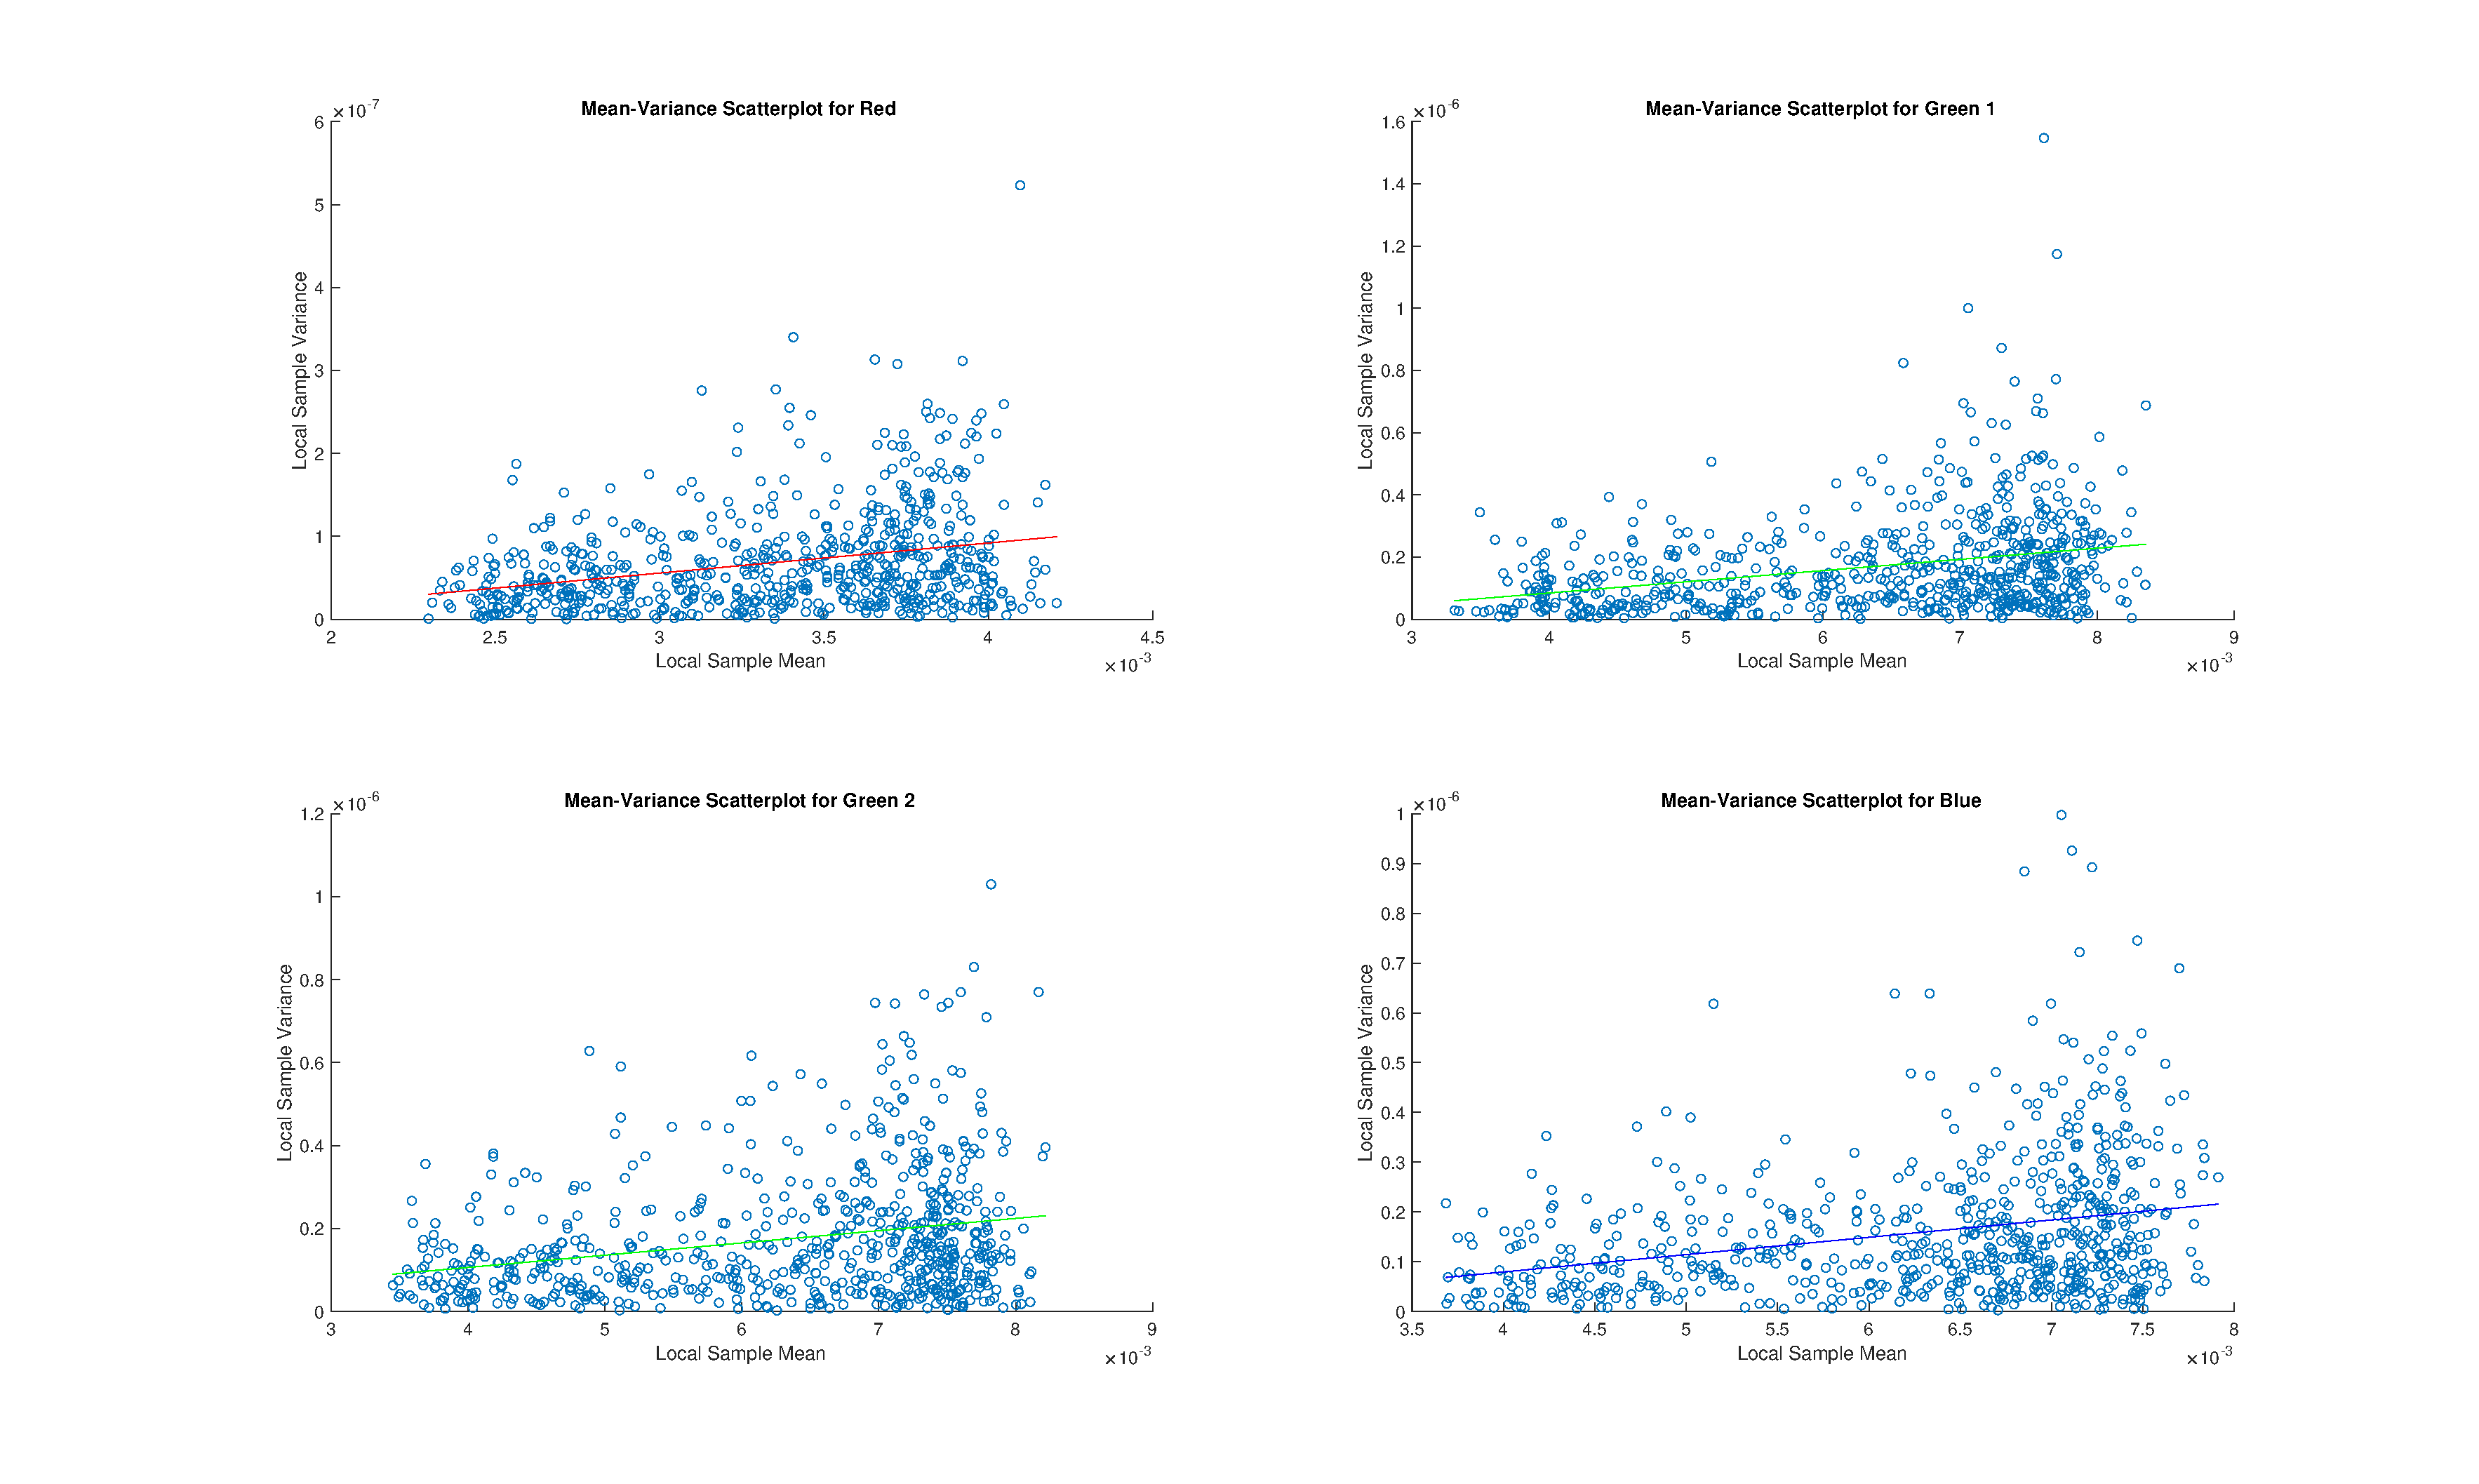
\includegraphics[width=\textwidth]{img/noisy-mean-variance.eps}
  \caption{Mean-variance for each channels before denoising}
  \label{fig:noisy-mean-variance}
\end{figure}

\begin{figure}
  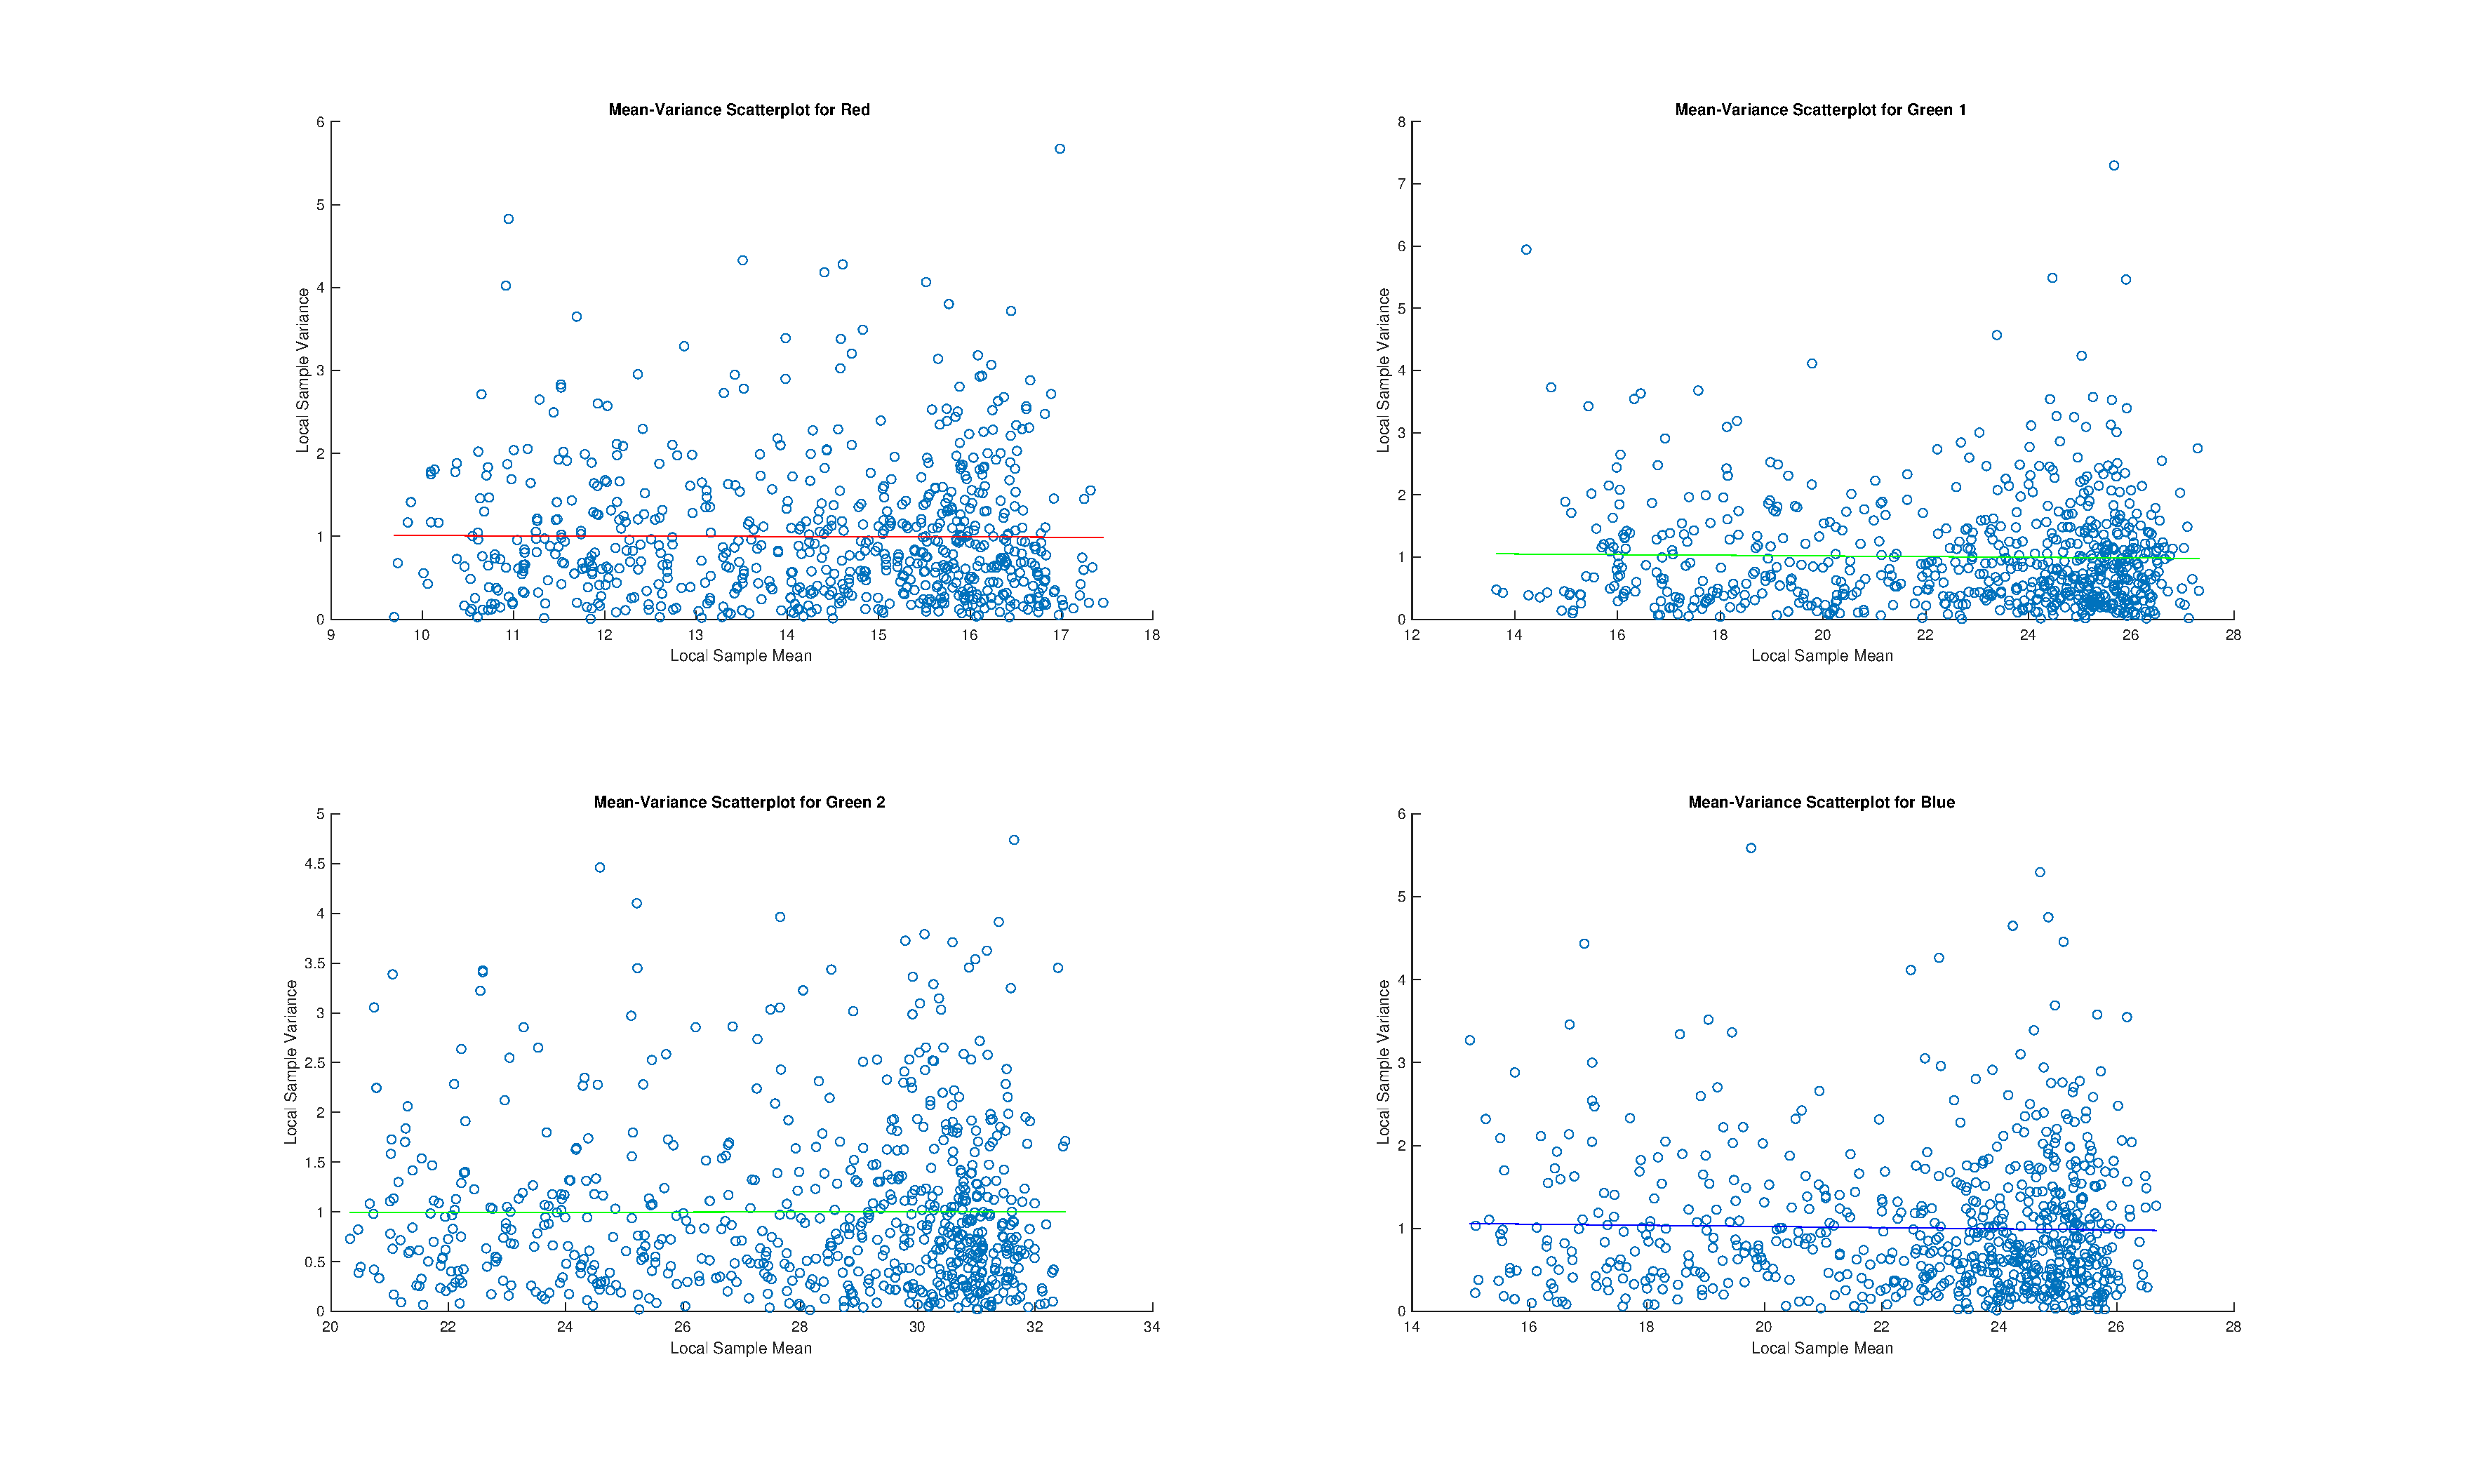
\includegraphics[width=\textwidth]{img/clean-mean-variance.eps}
  \caption{Mean-variance for each channels after denoising}
  \label{fig:clean-mean-variance}
\end{figure}

\section{Comparing non-transformed and transformed images}
After combining the channels to a RGB image we can compare the images produced when Poisson noise was removed and when it was not. Figure~\ref{fig:comparison-dct} shows the images produced by the pipeline without and with the Anscombe transformation. From these images we can see that the transformed image is clearly more detailed. From this we can conclude that the transformation greatly benefits the image formation pipeline, when using Bayer array sensor data.

\begin{figure}[h]
  \centering
  \begin{minipage}[b]{0.45\textwidth}
    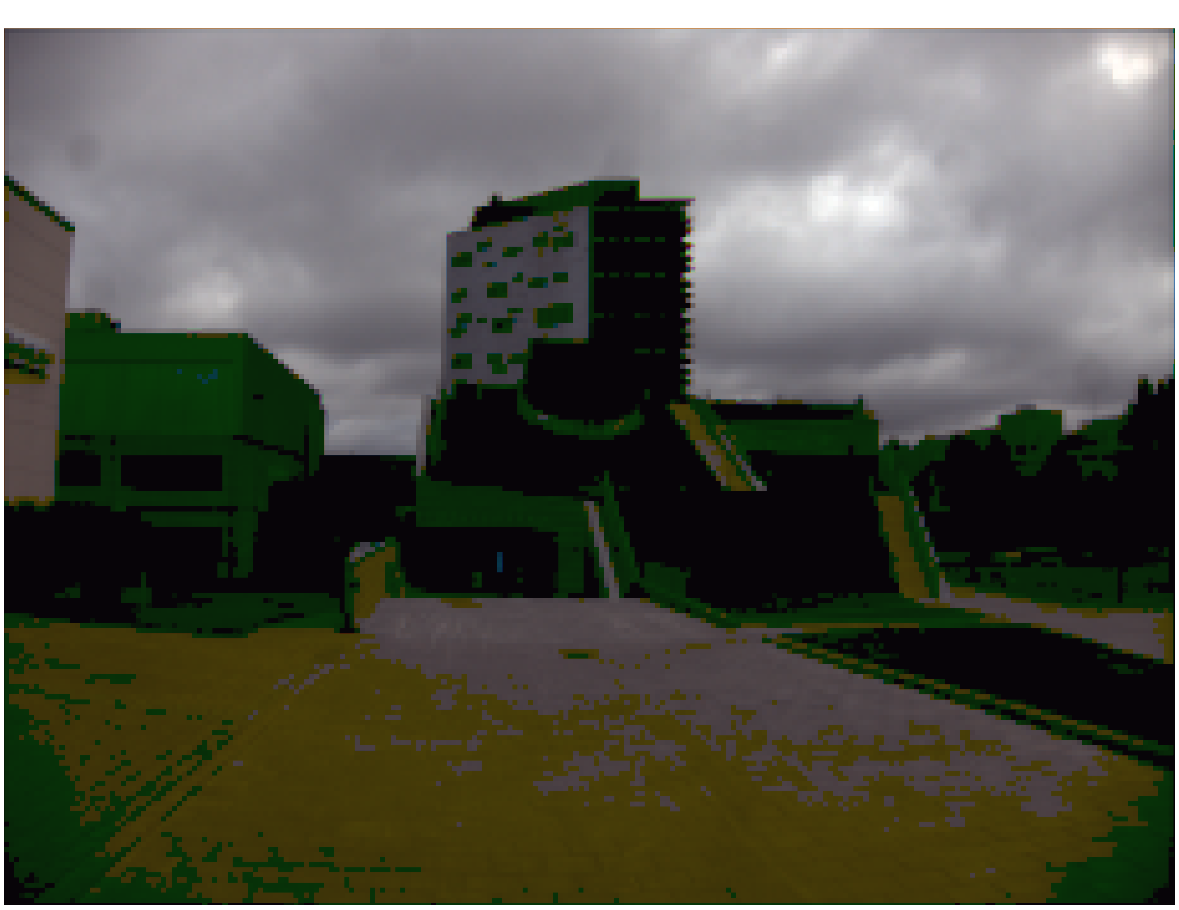
\includegraphics[width=\textwidth]{img/non-transformed-dct.png}
    \caption*{(a) Produced image withouth Anscombe transformation}
    %\label{fig:nontransformed-dct}
  \end{minipage}
  \hfill
  \begin{minipage}[b]{0.45\textwidth}
    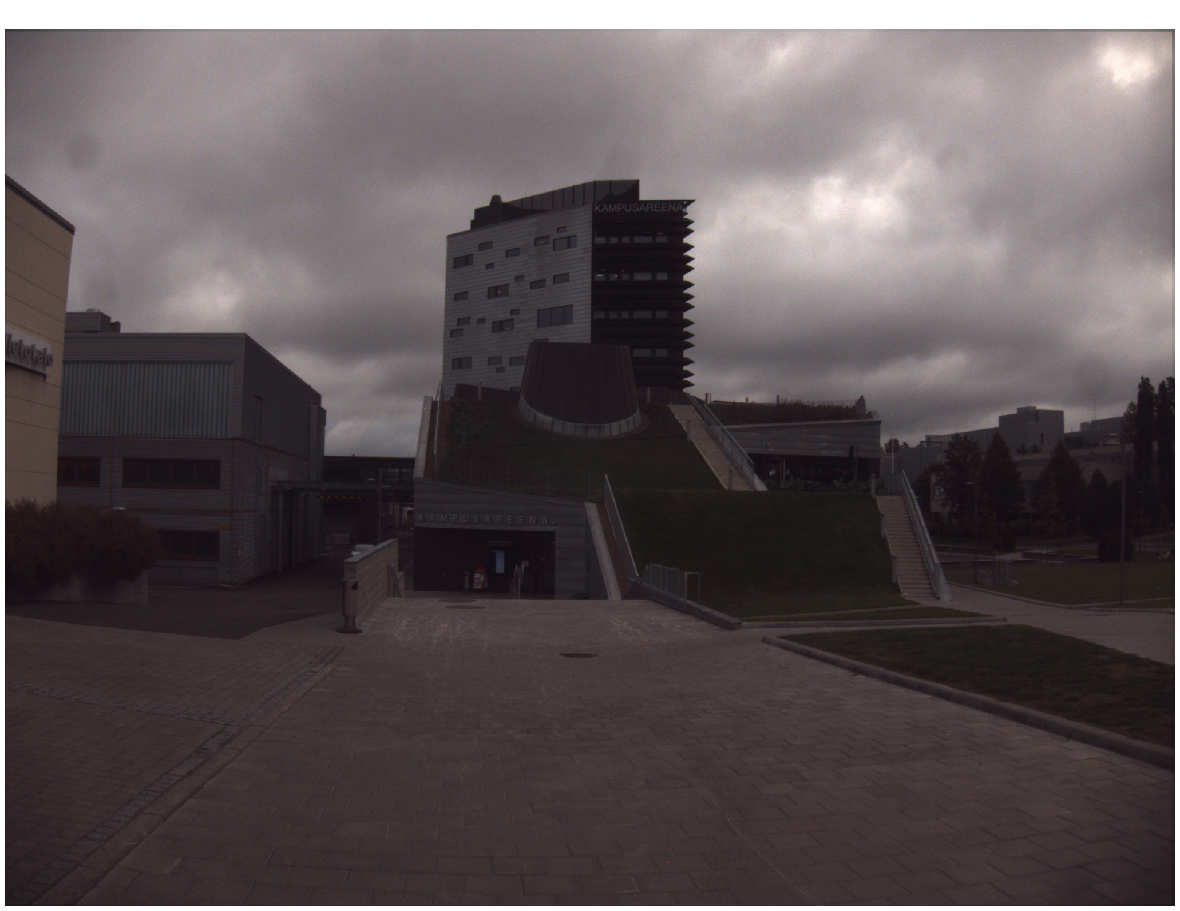
\includegraphics[width=\textwidth]{img/transformed-dct.png}
    \caption*{(b) Produced image with Anscombe transformation}
    %\label{fig:transformed-dct}
  \end{minipage}
  \caption{Comparision of images where (a) was not applied Anscombe transformation before reconstruction, and (b) as applied Anscombe transformation.}
  \label{fig:comparison-dct}
\end{figure}

\section{Color correction}
After producing RGB we applied white balancing, saturation correction and contrast correction. Figure~\ref{fig:comparison-white-balance} shows the difference between the images that have not and were applied Anscombe transformation before RGB composition after white balancing, saturation and contrast corrections. The non-transformed image is a lot brighter but it is still unclear. The transformed image still looks good, as it's somewhat brighter. By eye it also looks like with the chosen lambda value the green color has been reduced somewhat, which might not be wanted.

\begin{figure}[h]
  \centering
  \begin{minipage}[b]{0.45\textwidth}
    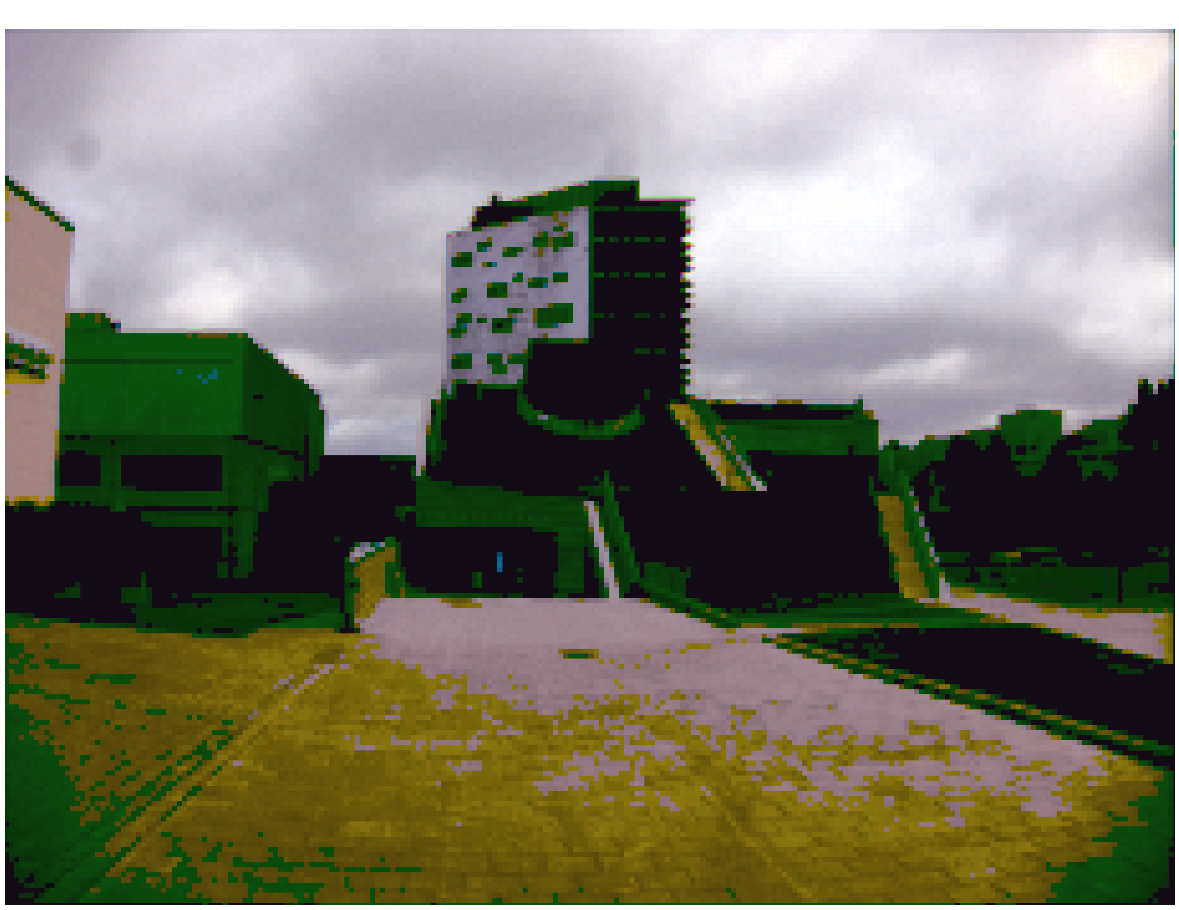
\includegraphics[width=\textwidth]{img/non-transformed-white-balance.png}
    \caption*{(a) Produced image withouth Anscombe transformation after color correction}
    %\label{fig:nontransformed-dct}
  \end{minipage}
  \hfill
  \begin{minipage}[b]{0.45\textwidth}
    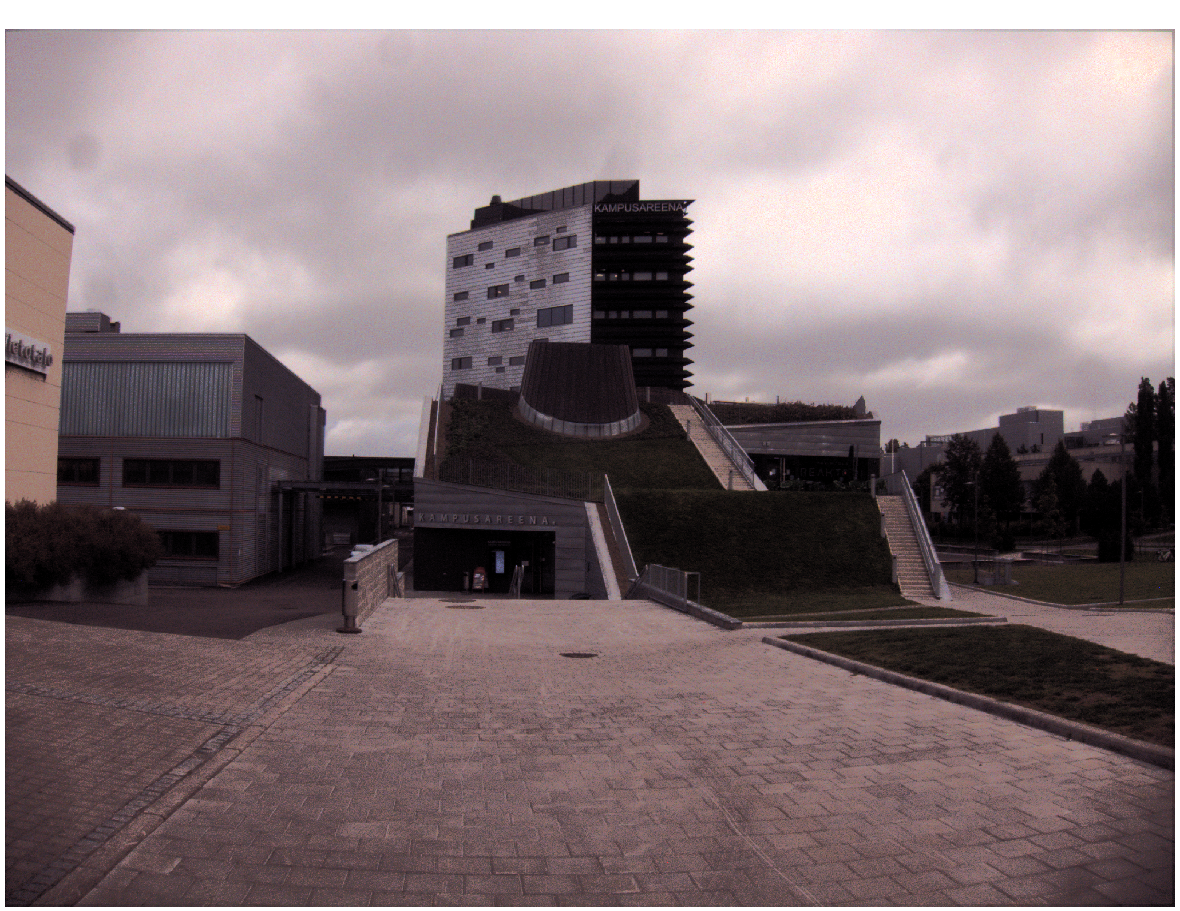
\includegraphics[width=\textwidth]{img/transformed-white-balance.png}
    \caption*{(b) Produced image with Anscombe transformation after color connection}
    %\label{fig:transformed-dct}
  \end{minipage}
  \caption{Comparision of images where (a) was not applied Anscombe transformation before reconstruction, and (b) as applied Anscombe transformation.}
  \label{fig:comparison-white-balance}
\end{figure}


\chapter{Conclusions}
\label{ch:conclusions}
%
% The bibliography, i.e the list of references
%
\newpage

\printbibliography[title=References]
\addcontentsline{toc}{chapter}{References}

\end{document}

